\documentclass{article}

\usepackage{graphicx}
\usepackage[hidelinks]{hyperref}
\usepackage[a4paper, total={6in, 8in}]{geometry}
\usepackage[slovak]{babel}
\usepackage{caption}
\usepackage{subcaption}
\usepackage{listings}

\graphicspath{./include/}

\renewcommand{\figurename}{Obr.}
\renewcommand{\contentsname}{Obsah}

\begin{document}

\begin{titlepage}
	\null\vfill

	\begin{center}
		{\Huge Identifikácia servosystému }
		\vskip 2cm

		{\Large Cvičenie č. 7}
		\vskip 0.5cm

		{\large Spojité procesy}
	\end{center}

	\vfill
	\vfill

	\begin{flushright}
		Filip Lobpreis \\
		Matúš Machata \\
		\small\today\\
	\end{flushright}
	\hfill
\end{titlepage}

\thispagestyle{empty}
\clearpage

\tableofcontents
\thispagestyle{empty}
\clearpage

\section{Zadanie}
\label{sec:zadanie}
\pagenumbering{arabic}

\begin{figure}[!htbp]
	\begin{center}
		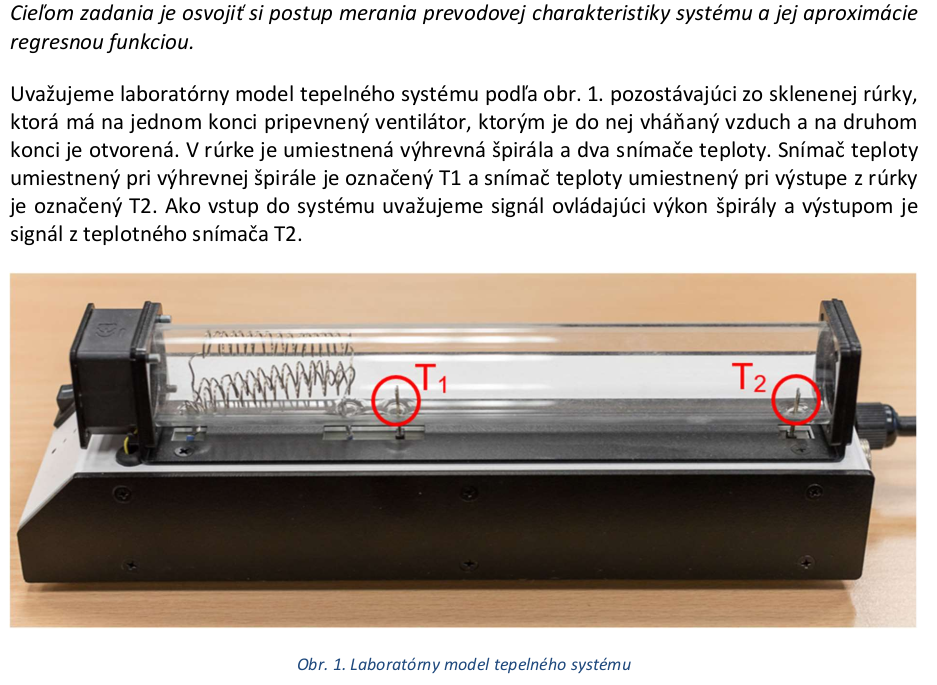
\includegraphics[width=0.8\textwidth]{./include/zadanie.png}
	\end{center}
	\caption{Zadania z~cvičenia č. 7 z~predmetu spojité procesy.}
	\label{fig:zadanie1}
\end{figure}

\clearpage

\section{Teória}
\label{sec:teoria}

Zadanie č. 7 sa zaoberá identifikáciou servosystému v~predurčenom pracovnom bode $U_0$.

\begin{figure}[!htbp]
	\begin{center}
		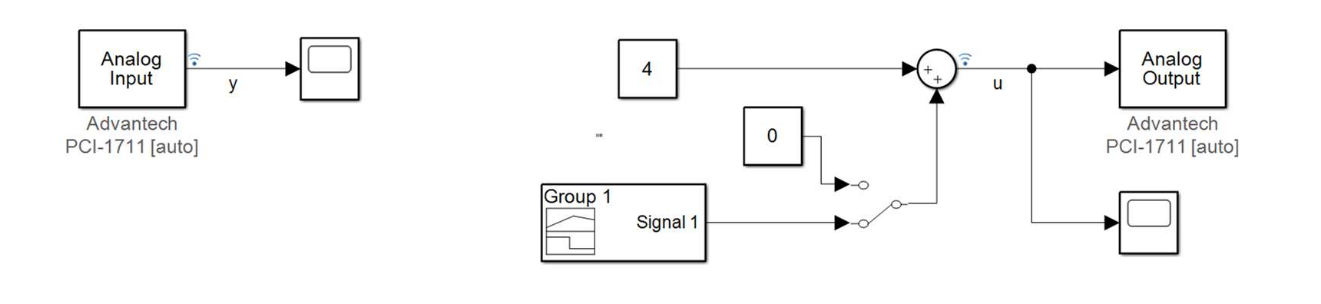
\includegraphics[width=0.95\textwidth]{include/schema.png}
	\end{center}
	\caption{Schéma zapojenia vstupu servosystému.}
	\label{fig:schema}
\end{figure}

Ako prvú vec si potrebujeme určiť hodnotu otáčok v~pracovnom bode. Ten máme preddefinovaný na~4V. Ako druhú vec budeme
zisťovať prenosovú funkciu, ktorá čo najpresnejšie opisuje nameraný graf. Vstupný signál pre~druhu úlohu vidíme na
obrázku.

\clearpage

\subsection{Uloha 1}
\label{subsec:u1}

Našou prvou úlohou ako už~bolo spomenuté v~\ref{sec:teoria} je nájsť pracovný bod. Predpísanú vstupnú hodnotu máme
$U_0 = 4V$. Tuto hodnotu sme mali už~prednastavenú v~simulácii \ref{fig:schema}. Simuláciu sme preto~spustili
a~odčítali sme ustálenú hodnotu z~grafu. Vstupný a~výstupný signál je zaznamenávaný s~periódou vzorkovania 0.01s.

Pri~vstupe $U_0 = 4V$ sme dostali na~výstupe rýchlosť otáčok $Y_0 = 6,8986$. Vstupný signál vidíme na~obrázku
Obr.~\ref{fig:uloha1_graf}

\begin{figure}[!htbp]
	\begin{center}
		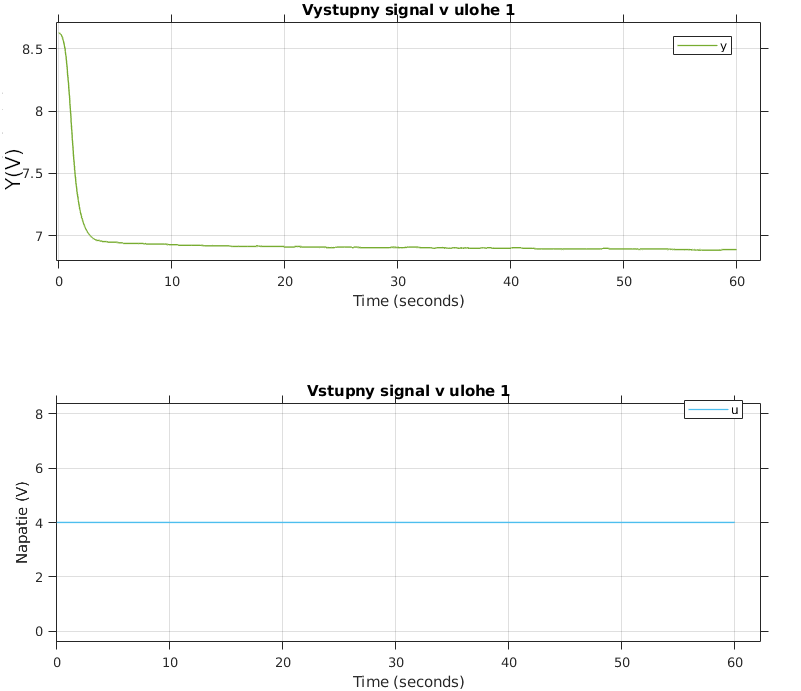
\includegraphics[width=0.95\textwidth]{include/uloha1_graf.png}
	\end{center}
	\caption{Vstupný a~výstupný signál prvej úlohy.}
	\label{fig:uloha1_graf}
\end{figure}

\clearpage

\section{Uloha 2}
\label{subsec:u2}

Na~začiatku druhej úlohy sme museli v~schéme prepnúť prepínač vstupného konštantného\\
signálu na~obdĺžnikový signál, ktorý sa pohybuje v~okolí pracovného bodu 4V s~amplitúdou 0.5V
(Obr.~\ref{fig:vstup2}). Perióda zmeny signálu je 10s. Podobne ako v~prvej úlohe,
perióda vzorkovania vstupného a~výstupného signálu je 0.01s.

\begin{figure}[!htbp]
	\begin{center}
		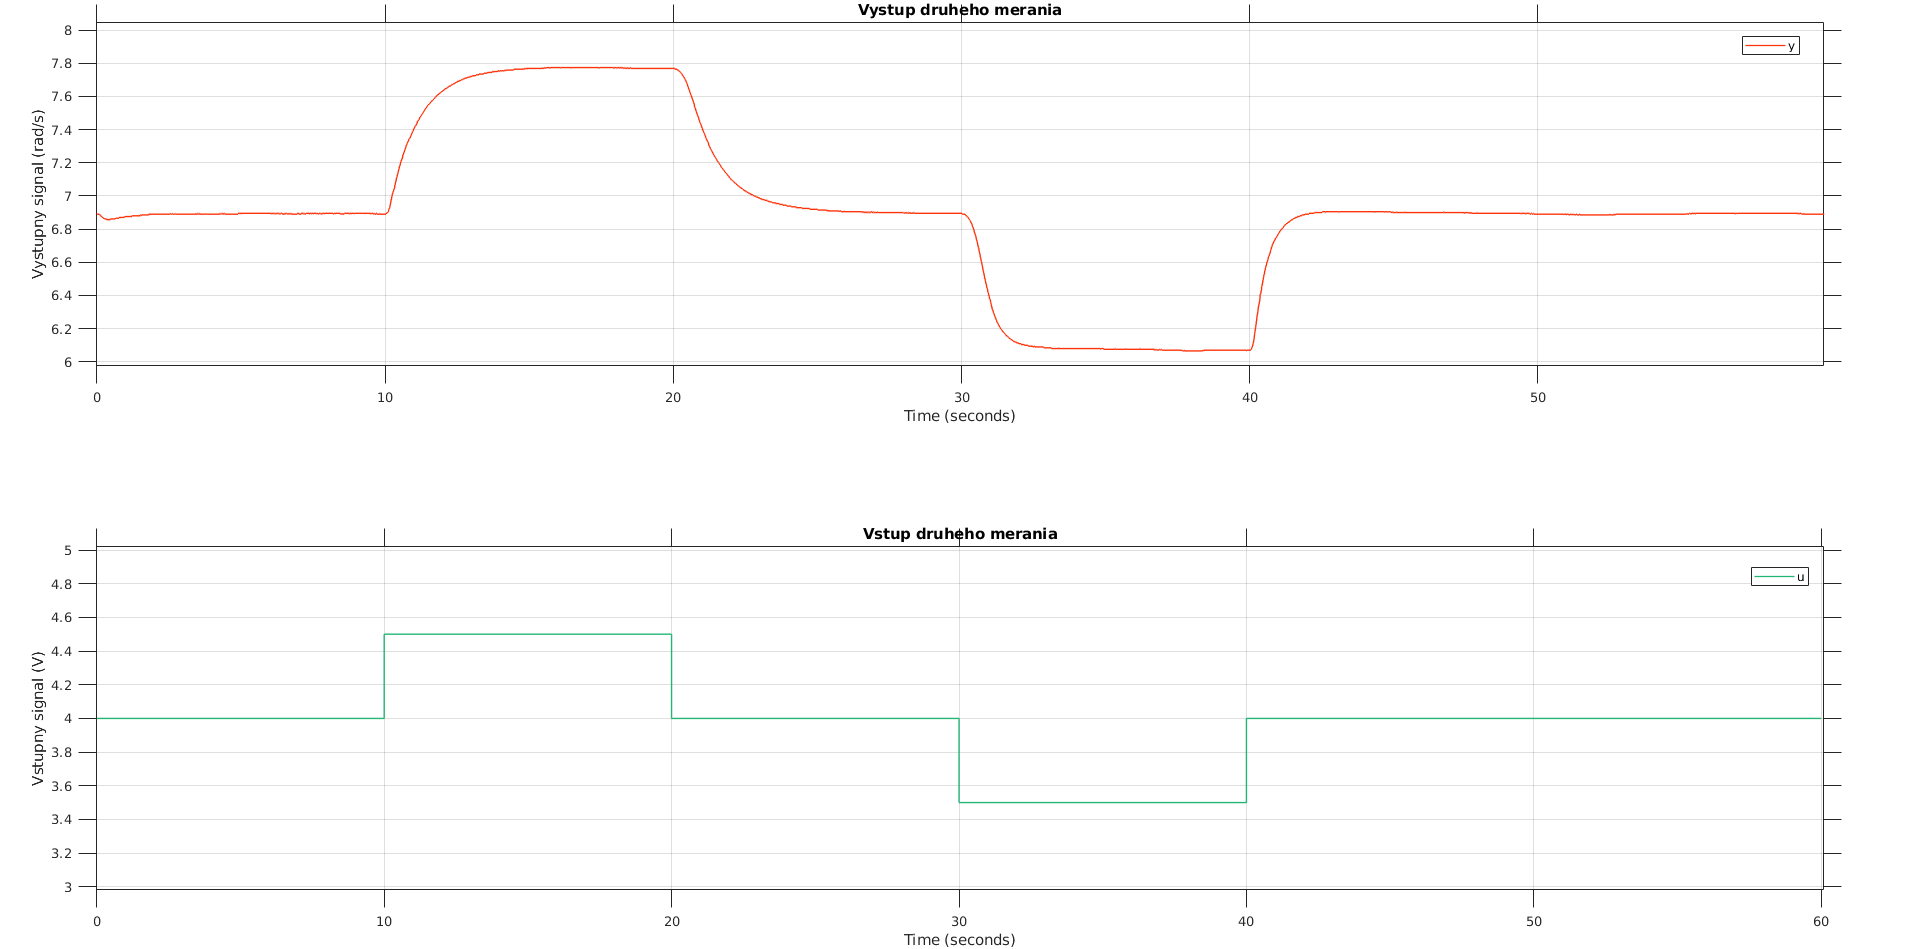
\includegraphics[width=0.95\textwidth]{include/vstup2_2.png}
	\end{center}
	\caption{Graf vstupného signálu do~servosystému v~úlohe 2.}
	\label{fig:vstup2}
\end{figure}

Identifikácia sa v~simulačnom prostredí MATLAB vykonáva pomocou funkcie \textbf{arx}.
Vstupne parametre tejto funkcie sú: 
\begin{itemize}
	\item matica vzorkovaných vstupno výstupných údajov
	\item vektor rádov
	\begin{itemize}
		\item čitateľa $n_a$
		\item menovateľa $n_b$
		\item dopravného oneskorenia $n_k$
	\end{itemize}
\end{itemize}

Aby sme zistili, ktorá identifikácia vychádza najlepšie. Počítame si sumu kvadrátu odchýliek medzi nameranou hodnotou
a~simulovanou hodnotou. Na~výpočet používame nasledovný vzťah:

\begin{equation}
	e = \sum_{i=0}^{i=N} (y_i - y_{si})^2
	\label{eq:odchylka}
\end{equation}
kde~$N$ je počet nameraných dát, $y$ sú~merane dáta a~$y_s$ sú~simulované dáta.

\clearpage

\subsection{Prvá identifikácia}
\label{subsec:I1}

Vstupné parametre rádov navrhovanej prenosovej funkcie sú:

\begin{lstlisting}[language=Matlab]
	na = 1;
	nb = 1;
	nk = 1;
\end{lstlisting}

\begin{figure}[!htbp]
	\begin{center}
		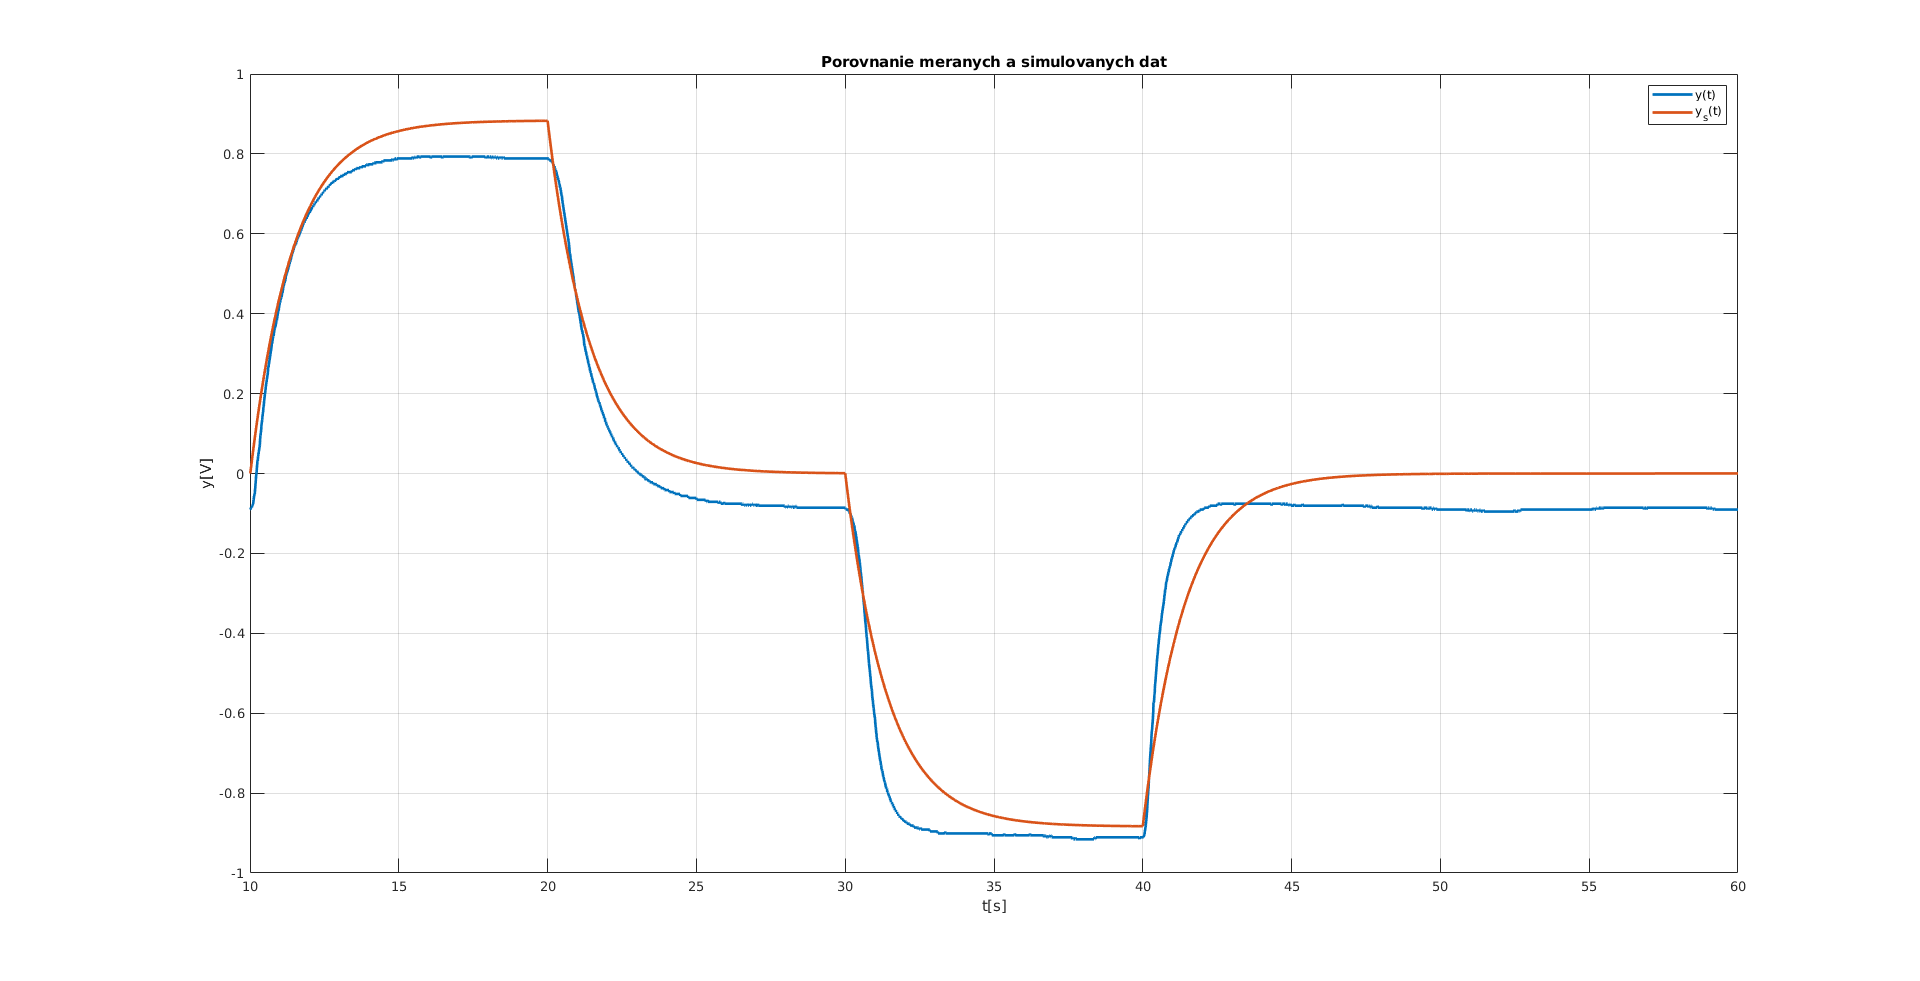
\includegraphics[width=0.95\textwidth]{include/I1.png}
	\end{center}
	\caption{Prvá identifikácia v~úlohe 2.}
	\label{fig:I1}
\end{figure}

Výsledná prenosová funkcia je:

\begin{equation}
	G_1(z) = \frac{0.01239}{z - 0.993}
	\label{eq:I1}
\end{equation}

Odchýlka nám vyšla $e = 40,0690$

\clearpage

\subsection{Druhá identifikácia}
\label{subsec:I2}

Vstupné parametre rádov navrhovanej prenosovej funkcie sú:

\begin{lstlisting}[language=Matlab]
	na = 3;
	nb = 3;
	nk = 1;
\end{lstlisting}

\begin{figure}[!htbp]
	\begin{center}
		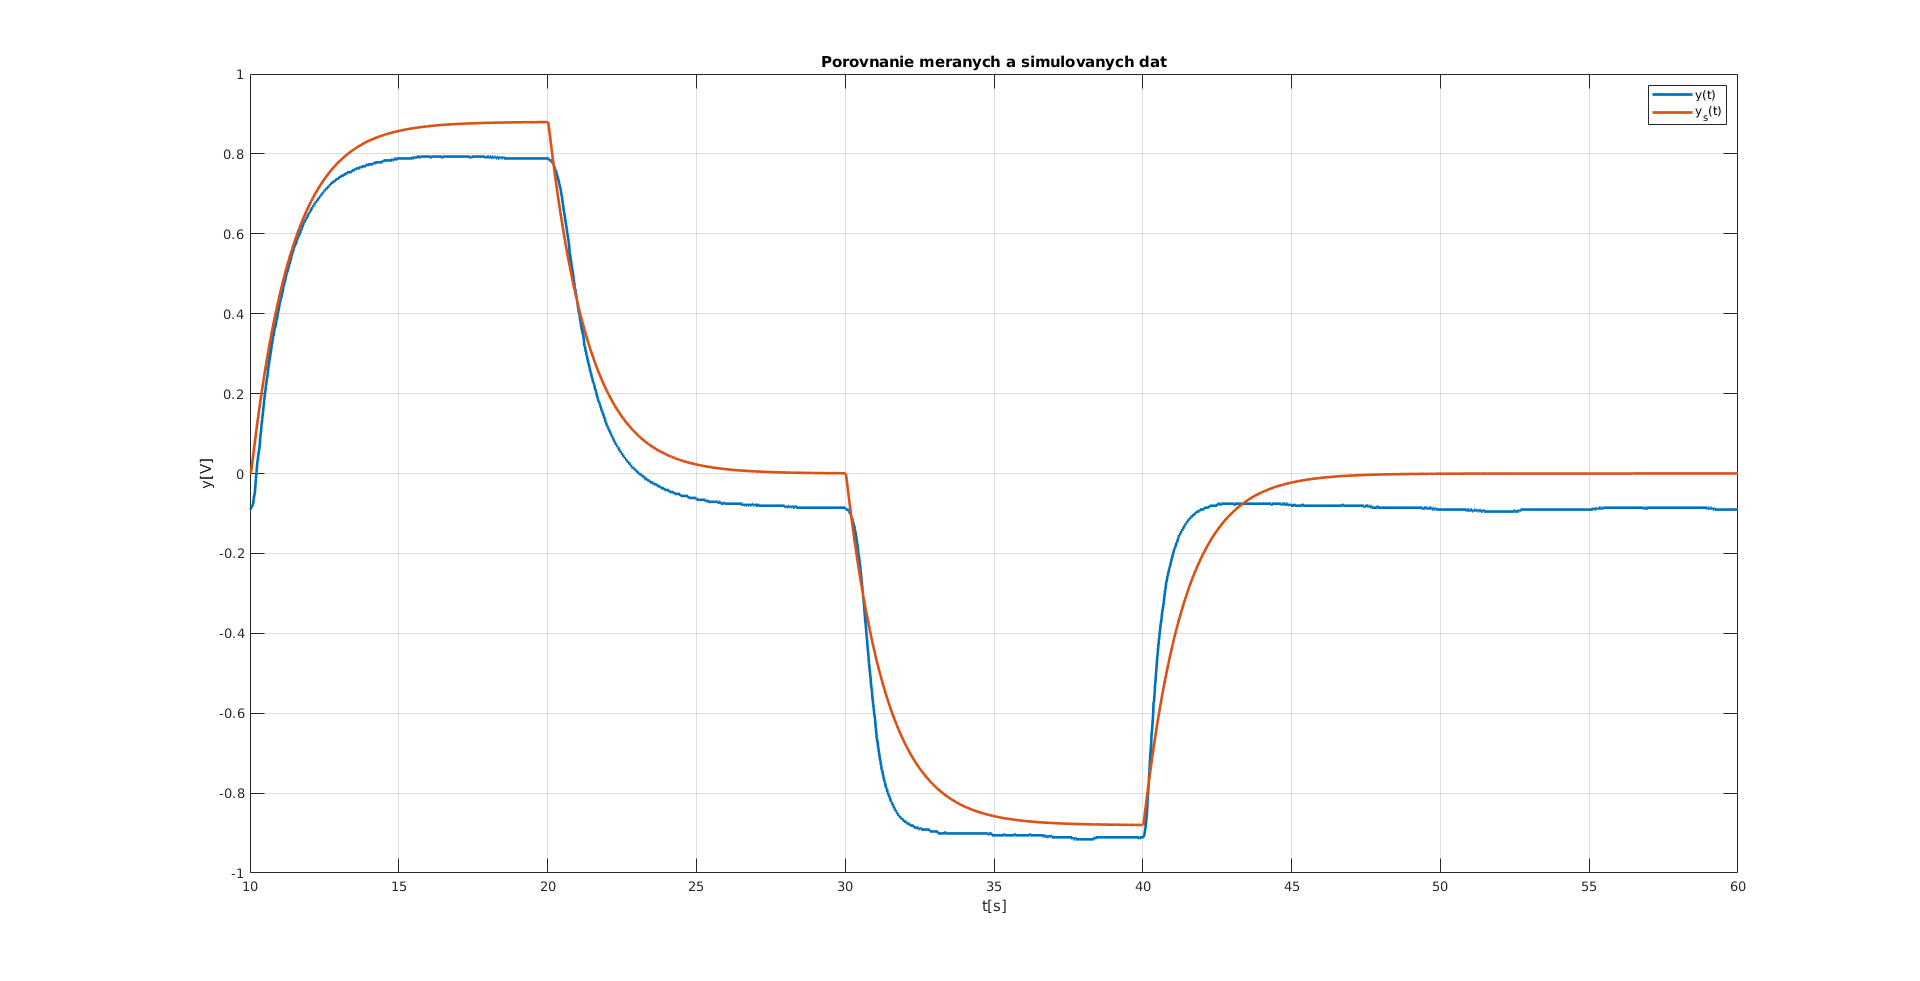
\includegraphics[width=0.95\textwidth]{include/I2.png}
	\end{center}
	\caption{Druhá identifikácia v~úlohe 2.}
	\label{fig:I2}
\end{figure}

Výsledná prenosová funkcia je:

\begin{equation}
	G_2(z) = \frac{0.0004583 z^2 + 0.003255 z + 0.004532}{z^3 - 1.026 z^2 - 0.2949 z + 0.3258}
	\label{eq:I2}
\end{equation}

Odchýlka nám vyšla $e = 38,2633$

\clearpage

\subsection{Tretia identifikácia}
\label{subsec:I3}

Vstupné parametre rádov navrhovanej prenosovej funkcie sú:

\begin{lstlisting}[language=Matlab]
	na = 4;
	nb = 1;
	nk = 1;
\end{lstlisting}

\begin{figure}[!htbp]
	\begin{center}
		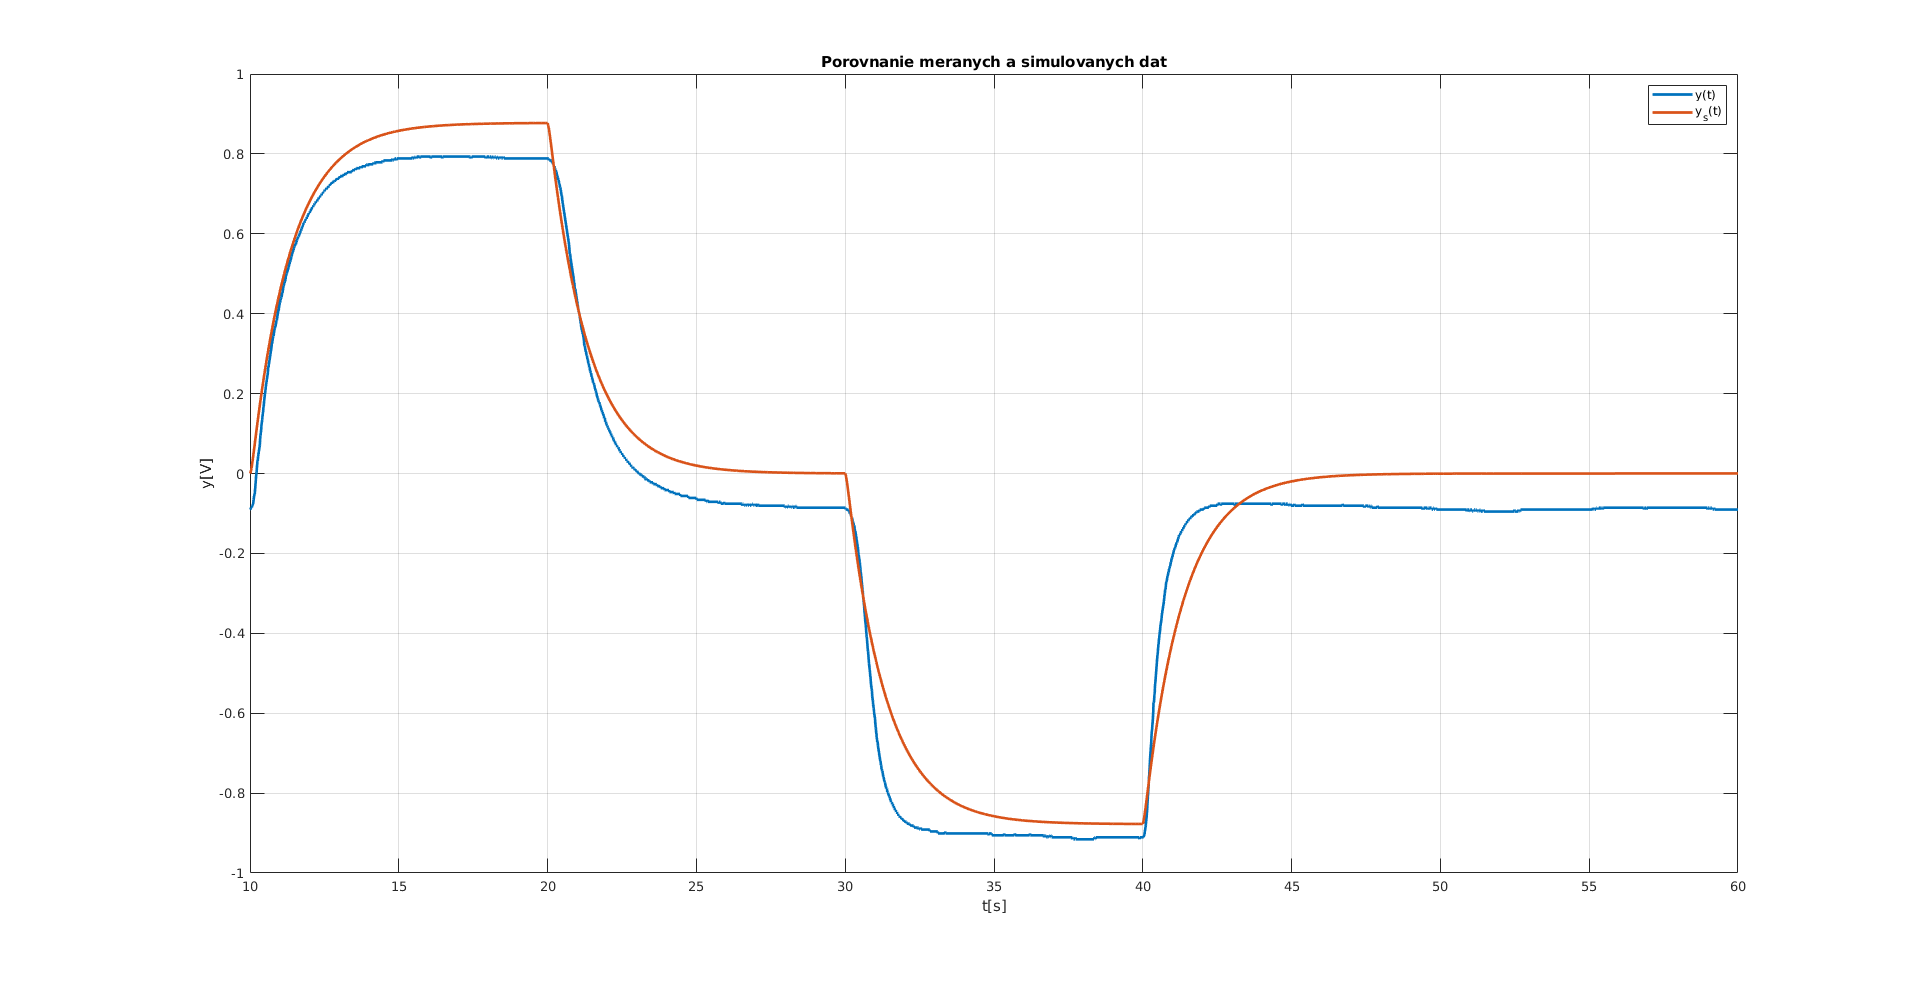
\includegraphics[width=0.95\textwidth]{include/I3.png}
	\end{center}
	\caption{Tretia identifikácia v~úlohe 2.}
	\label{fig:I3}
\end{figure}

Výsledná prenosová funkcia je:

\begin{equation}
	G_3(z) = \frac{0.005763}{z^4 - 0.9211 z^3 - 0.387 z^2 - 0.009722 z + 0.3212}
	\label{eq:I3}
\end{equation}

Odchýlka nám vyšla $e = 36,7178$.

\clearpage

\subsection{Štvrtá identifikácia}
\label{subsec:I4}

Vstupné parametre rádov navrhovanej prenosovej funkcie sú:

\begin{lstlisting}[language=Matlab]
	na = 8;
	nb = 1;
	nk = 1;
\end{lstlisting}

\begin{figure}[!htbp]
	\begin{center}
		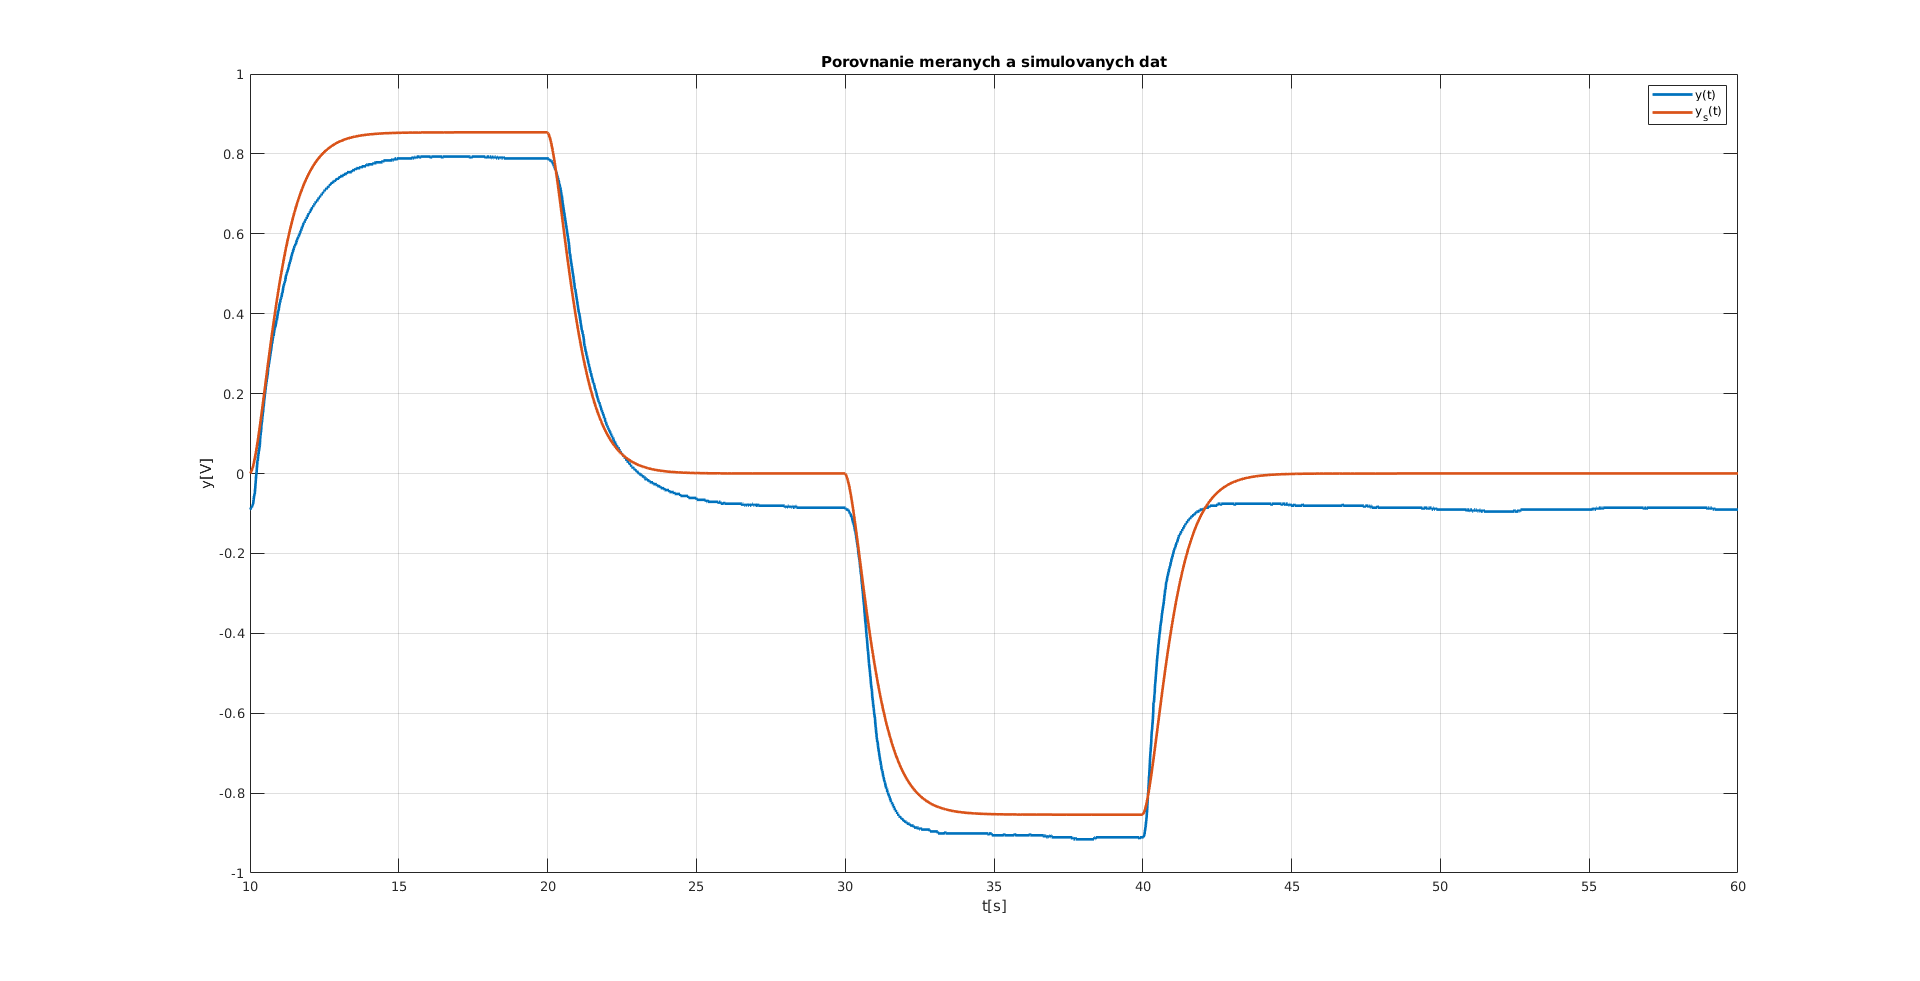
\includegraphics[width=0.95\textwidth]{include/I4.png}
	\end{center}
	\caption{Štvrtá identifikácia v~úlohe 2.}
	\label{fig:I4}
\end{figure}

Výsledná prenosová funkcia je:

\begin{equation}
	G_3(z) = \frac{0.003601}{z^8 - 0.6473 z^7 - 0.3345 z^6 - 0.1646 z^5 - 0.1028 z^4 - 0.05178 z^3 + 0.04753 z^2 + 0.07217 z + 0.1834}
	\label{eq:I4}
\end{equation}

Odchýlka nám vyšla $e = 30,3087$.

\clearpage

\subsection{Piata identifikácia}
\label{subsec:I5}

Vstupné parametre rádov navrhovanej prenosovej funkcie sú:

\begin{lstlisting}[language=Matlab]
	na = 8;
	nb = 5;
	nk = 1;
\end{lstlisting}

\begin{figure}[!htbp]
	\begin{center}
		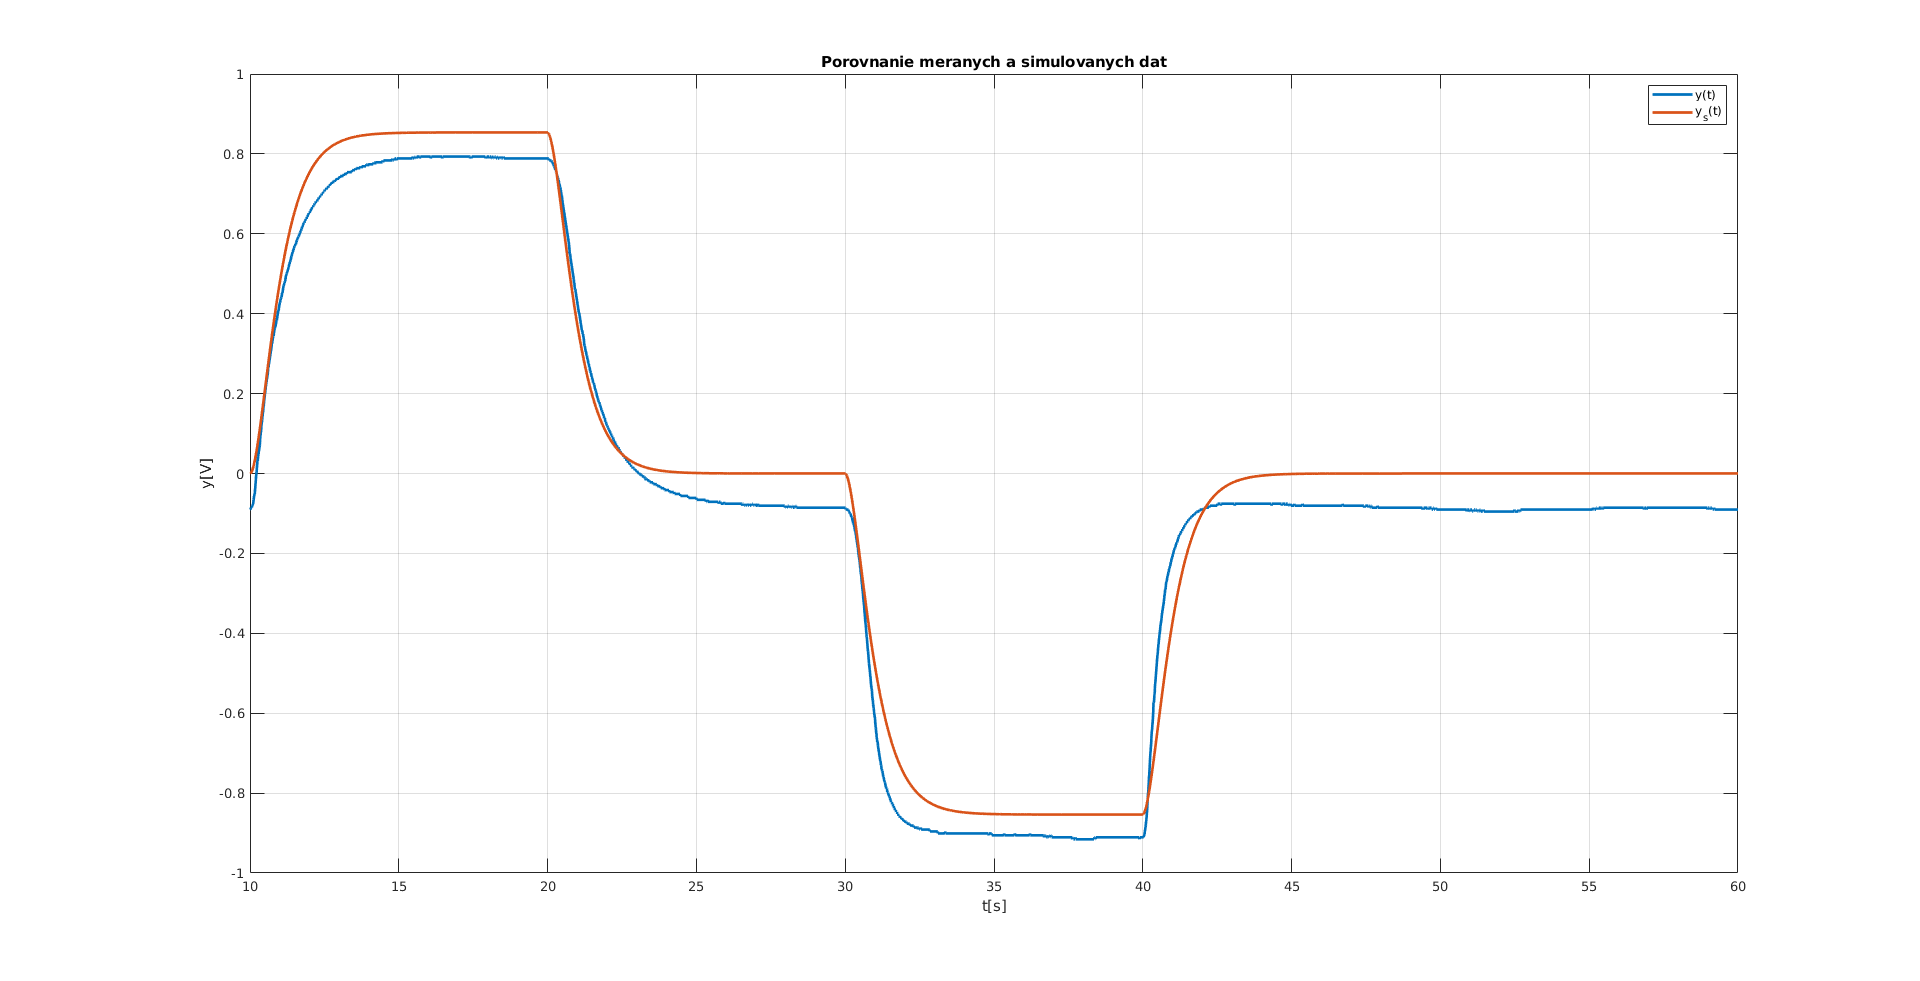
\includegraphics[width=0.95\textwidth]{include/I5.png}
	\end{center}
	\caption{Piata identifikácia v~úlohe 2.}
	\label{fig:I5}
\end{figure}

Výsledná prenosová funkcia je:

\begin{equation}
	G_5(z) = \frac{0.0001377 z^4 + 0.003255 z^3 - 0.002104 z^2 + 0.002169 z + 0.0003051}{z^8 - 0.6464 z^7 - 0.3338 z^6 - 0.1644 z^5 - 0.103 z^4 - 0.05215 z^3 + 0.0471 z^2 + 0.07177 z + 0.1831}
	\label{eq:I5}
\end{equation}

Odchýlka nám vyšla $e = 30,3875$.

\clearpage


\end{document}

